\documentclass[UTF8,a4paper,10pt,twocolumn]{article}

\usepackage{ctex}
\usepackage{physics}
\usepackage{graphicx} %
\usepackage[subfigure,AllowH]{graphfig} 

\title{基于Latex写作的大炮打蚊子研究}
\author{waacing}

\begin{document}
	\maketitle 
	我也不知道写啥随便写写。
	\section{公式}
	\subsection{公式对齐}
	运算过程/公式太长的运算符号对齐:
	\begin{equation} \label{}
		\begin{aligned}
			\frac{dG}{dt}&=\sum(\dot{\overline{r_i}}\cdot \overline{p_i} + \dot{\overline{p_i}} \cdot \overline{r_i} ) \\
			&=\sum(\overline{F_i}\cdot \overline{r_i} + \overline{p_i} \cdot \overline{v_i}) \\
			&=\sum(\overline{F_i}\cdot \overline{r_i} + mv_i^2)
		\end{aligned}
	\end{equation}
	 
	\subsection{大括号}
	\begin{equation}
		sample = \left\{ 
			\begin{aligned}
				r(t+\Delta t)&=r(t)+v(t)\Delta t+\frac{1}{2}a(t)\Delta t^2 \\
				v(t+\Delta t)&=v(t)+\frac{1}{2}[a(t)+a(t+\Delta t)]\Delta t
			\end{aligned}
		\right.
	\end{equation}
	
	\subsection{矩阵}
	
	\begin{equation} \label{Eq.HJ44}
		\begin{gathered}
			\begin{aligned}
				\begin{vmatrix} 
					\vb{i} & \vb{j} & \vb{k} \\ 
					v_x & v_y  & v_z \\ 
					u_x & u_y & u_z
				\end{vmatrix}
			\end{aligned}
		\end{gathered}
	\end{equation}
	
	\section{图片}
	\subsection{插入不用路径的图片}
	插入图片需要在文件顶部添加graphix包。
	
	{fig/force}表示读取存在fig文件夹中名为force的图片。请注意,不指出路径的话,Latex默认读取的是当前文件夹中的文件,不会进入到子文件夹中。使用了相对路径,就可以把所有要用到的图片都放在一个文件夹下,方便管理。
	
	%如果你的图片没有子图
	\begin{figure} [!h] % [!h]控制图片随着代码的位置改变
		\centering % 图片居中
		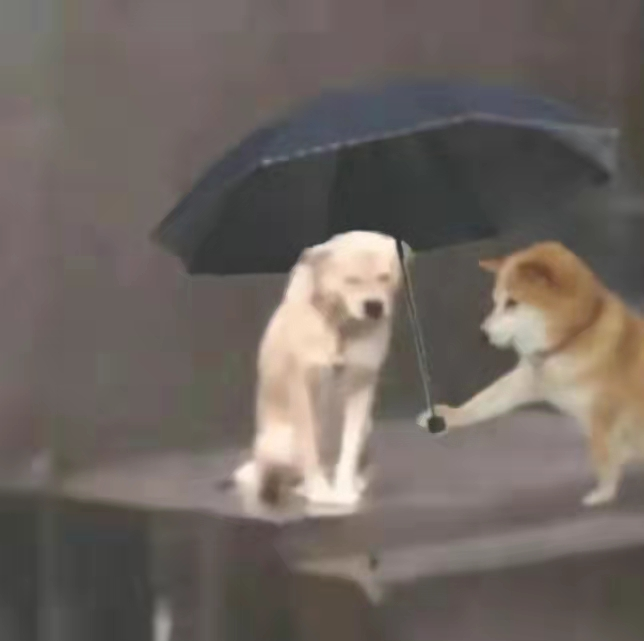
\includegraphics[width=0.7\linewidth]{fig/1} % 0.7\linewidth表示行距的0.7倍,fig/force表示读取存在fig文件夹中名为force的图片
		\caption{随便写写} %用来引用图片
	\end{figure}

	%如果你的图片有子图
	\begin{figure}[hb]
		\centering
		\subfigure[能量随温度变化关系图]{  % 子图的批注
			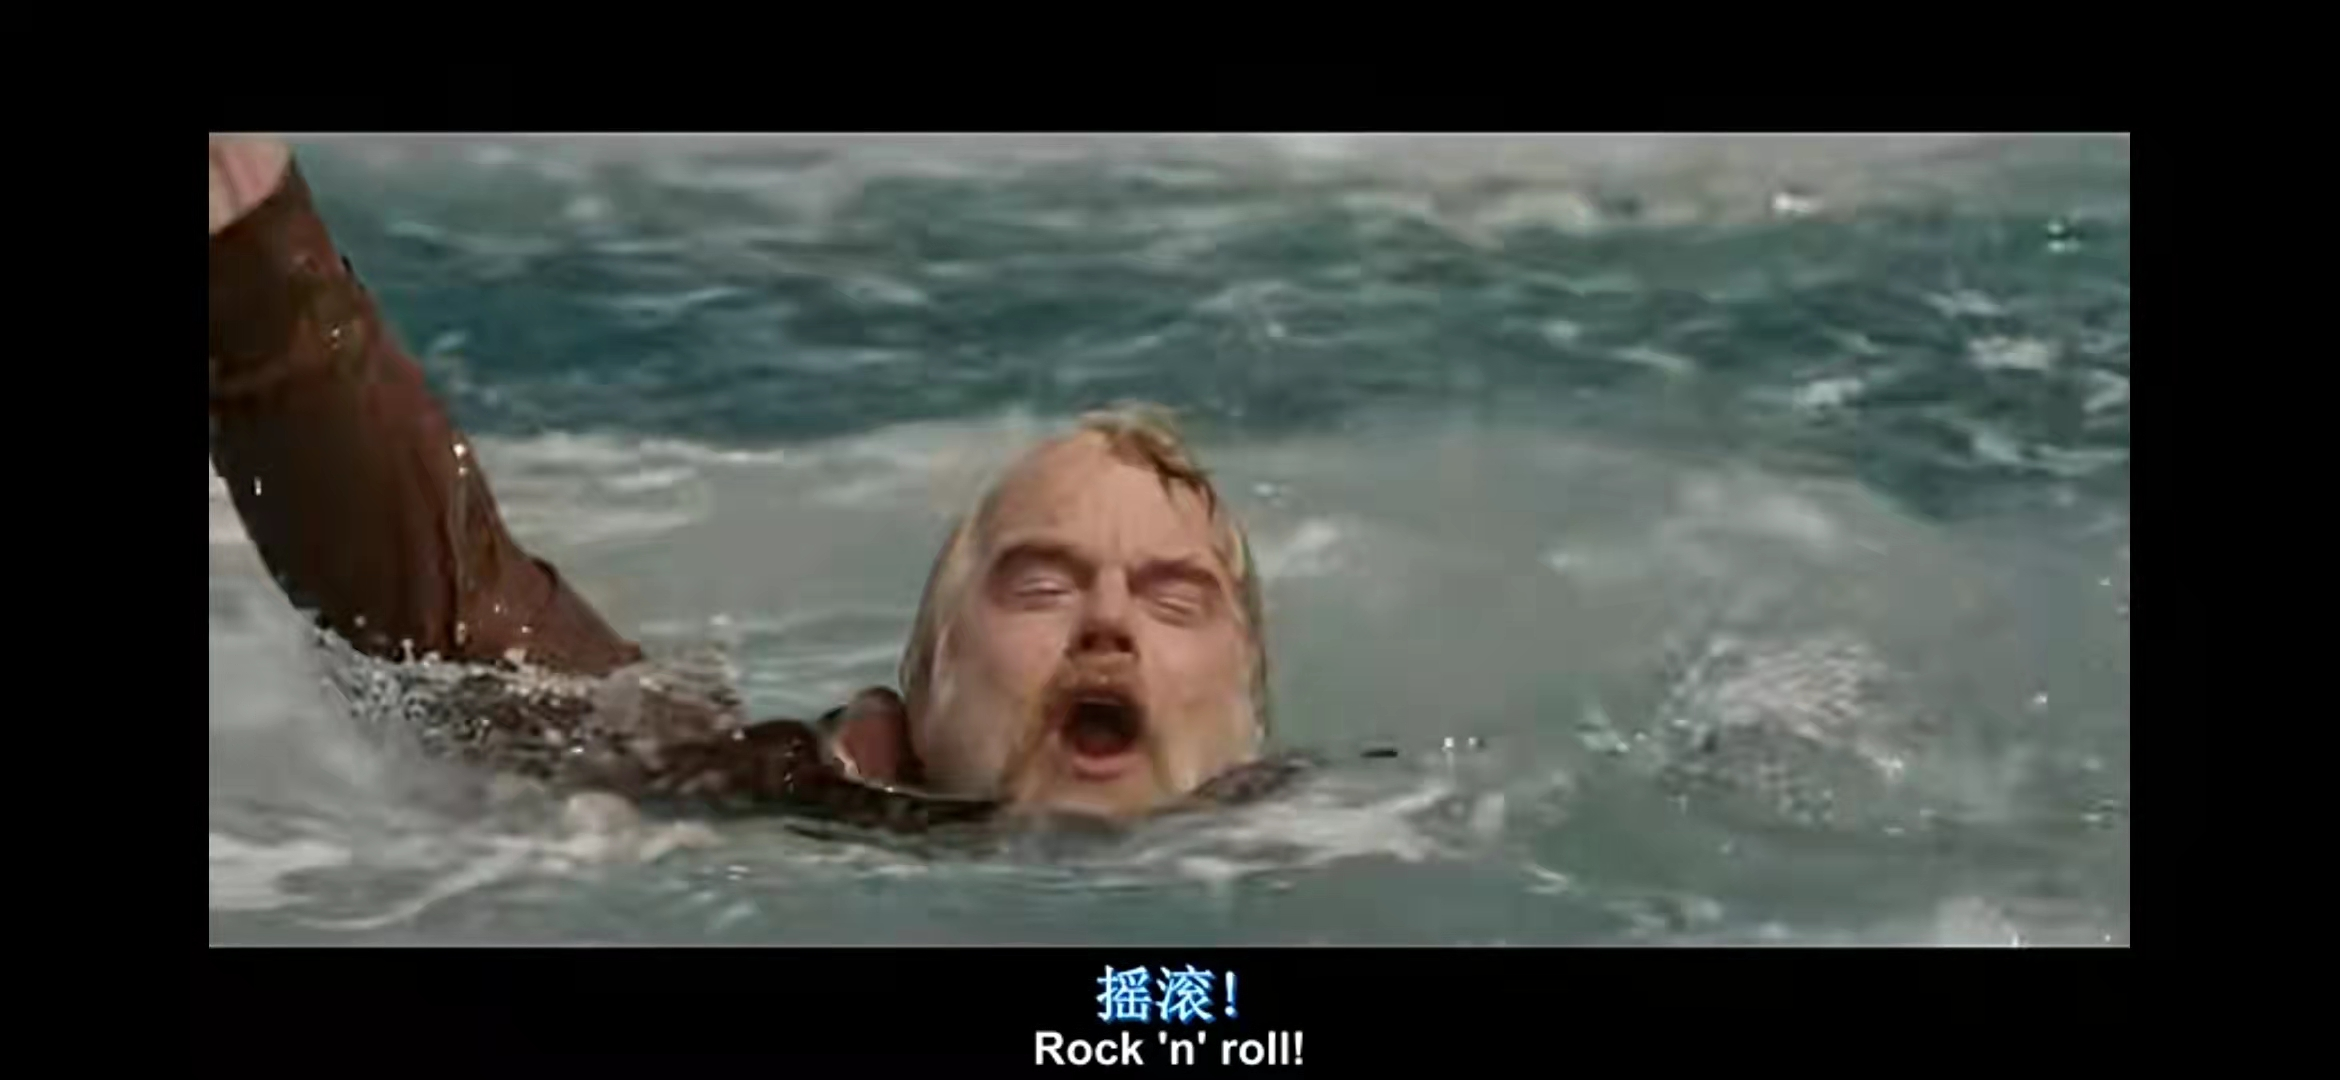
\includegraphics[scale=0.1]{fig/2} \label{1} %图形的缩放因子,设定 scale=0.2 会使插入的图形的大小为其自然大小的0.2倍。
		}
		\quad
		\subfigure[磁化强度与温度的关系图]{
			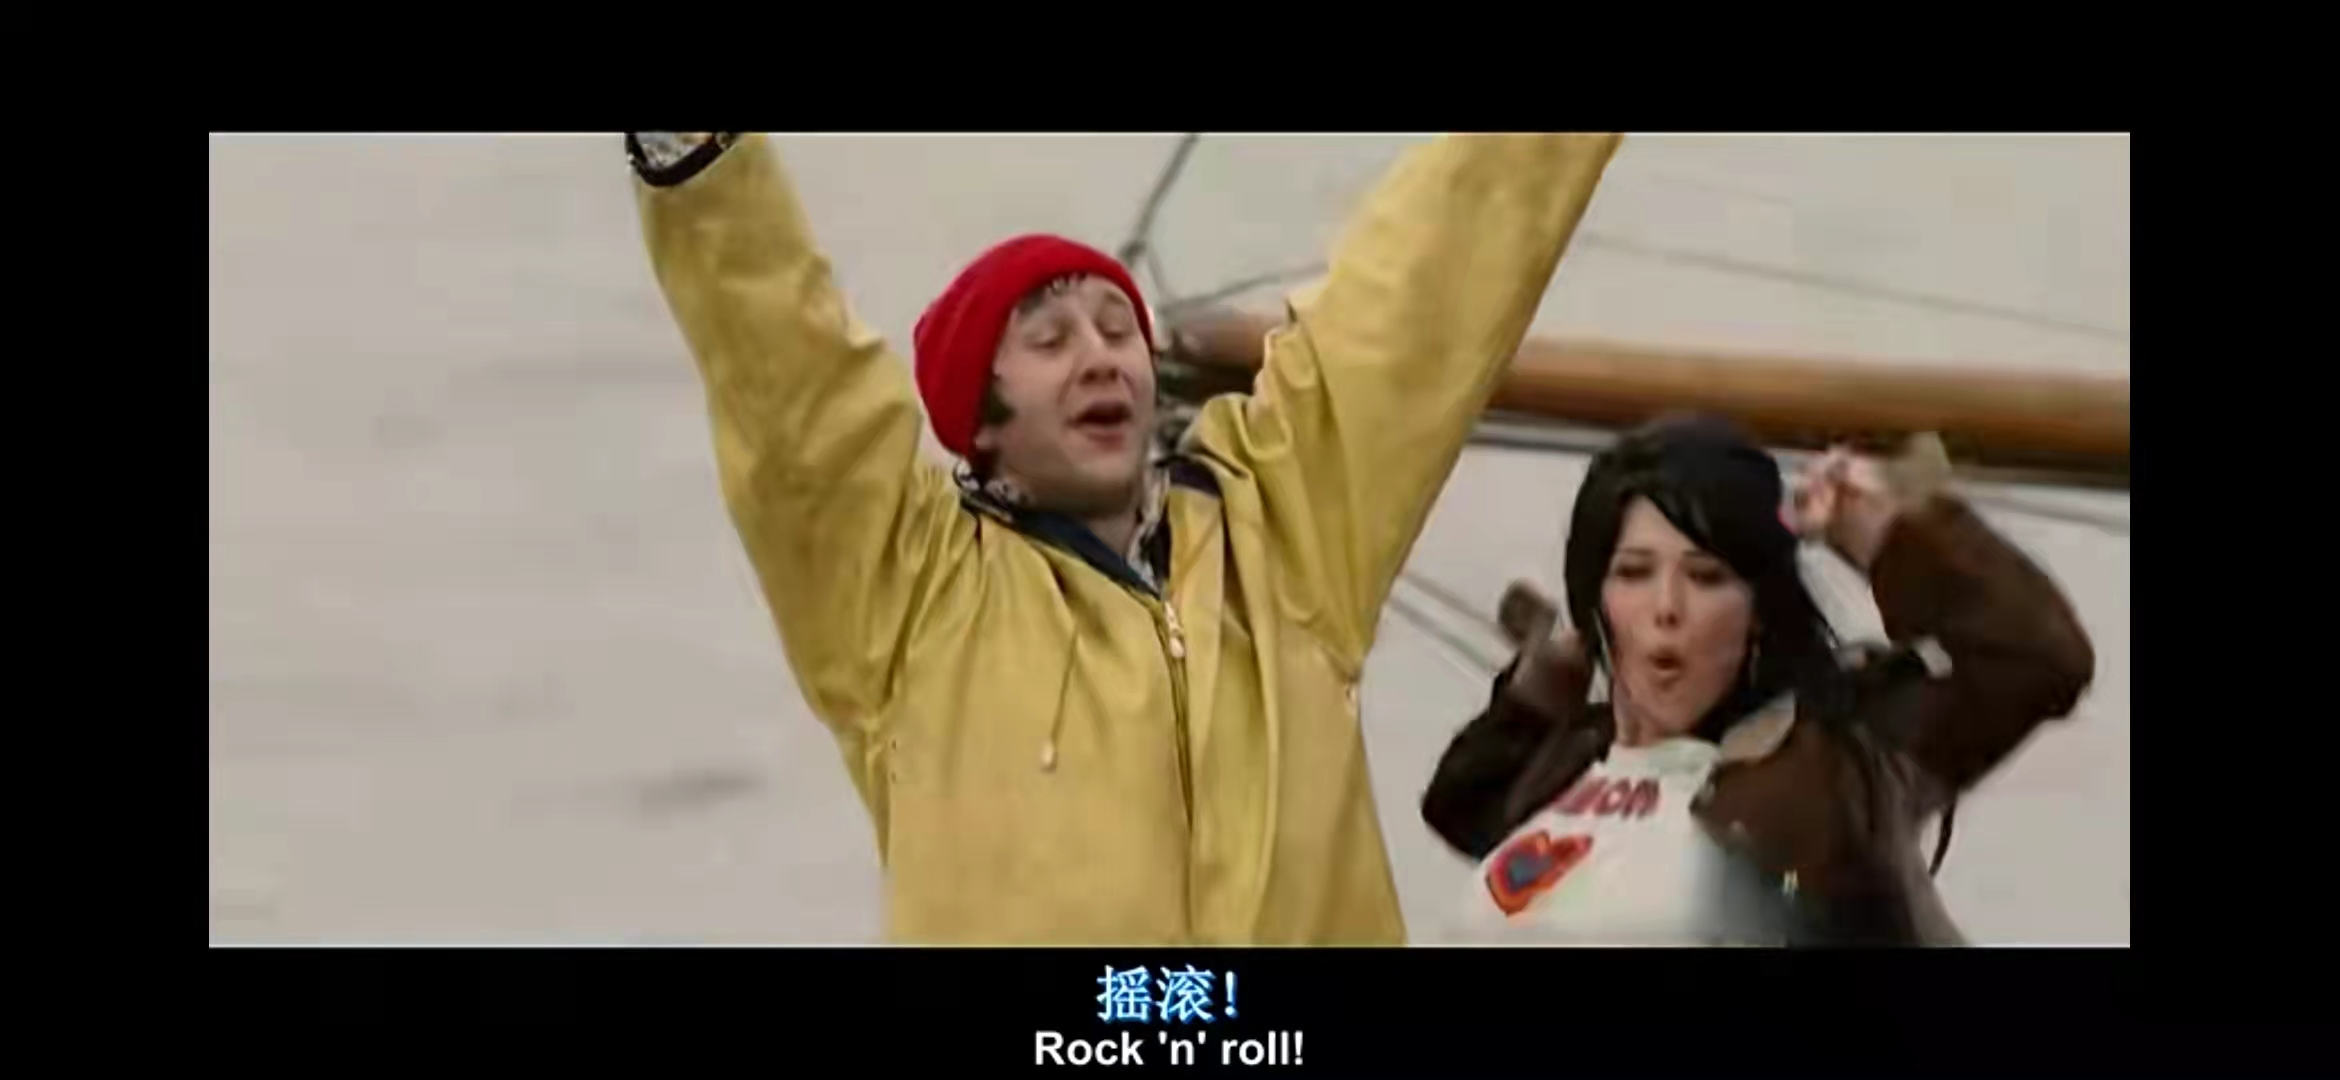
\includegraphics[scale=0.1]{fig/3} \label{2}
		}
		\quad
		\subfigure[热容与温度的关系图]{
			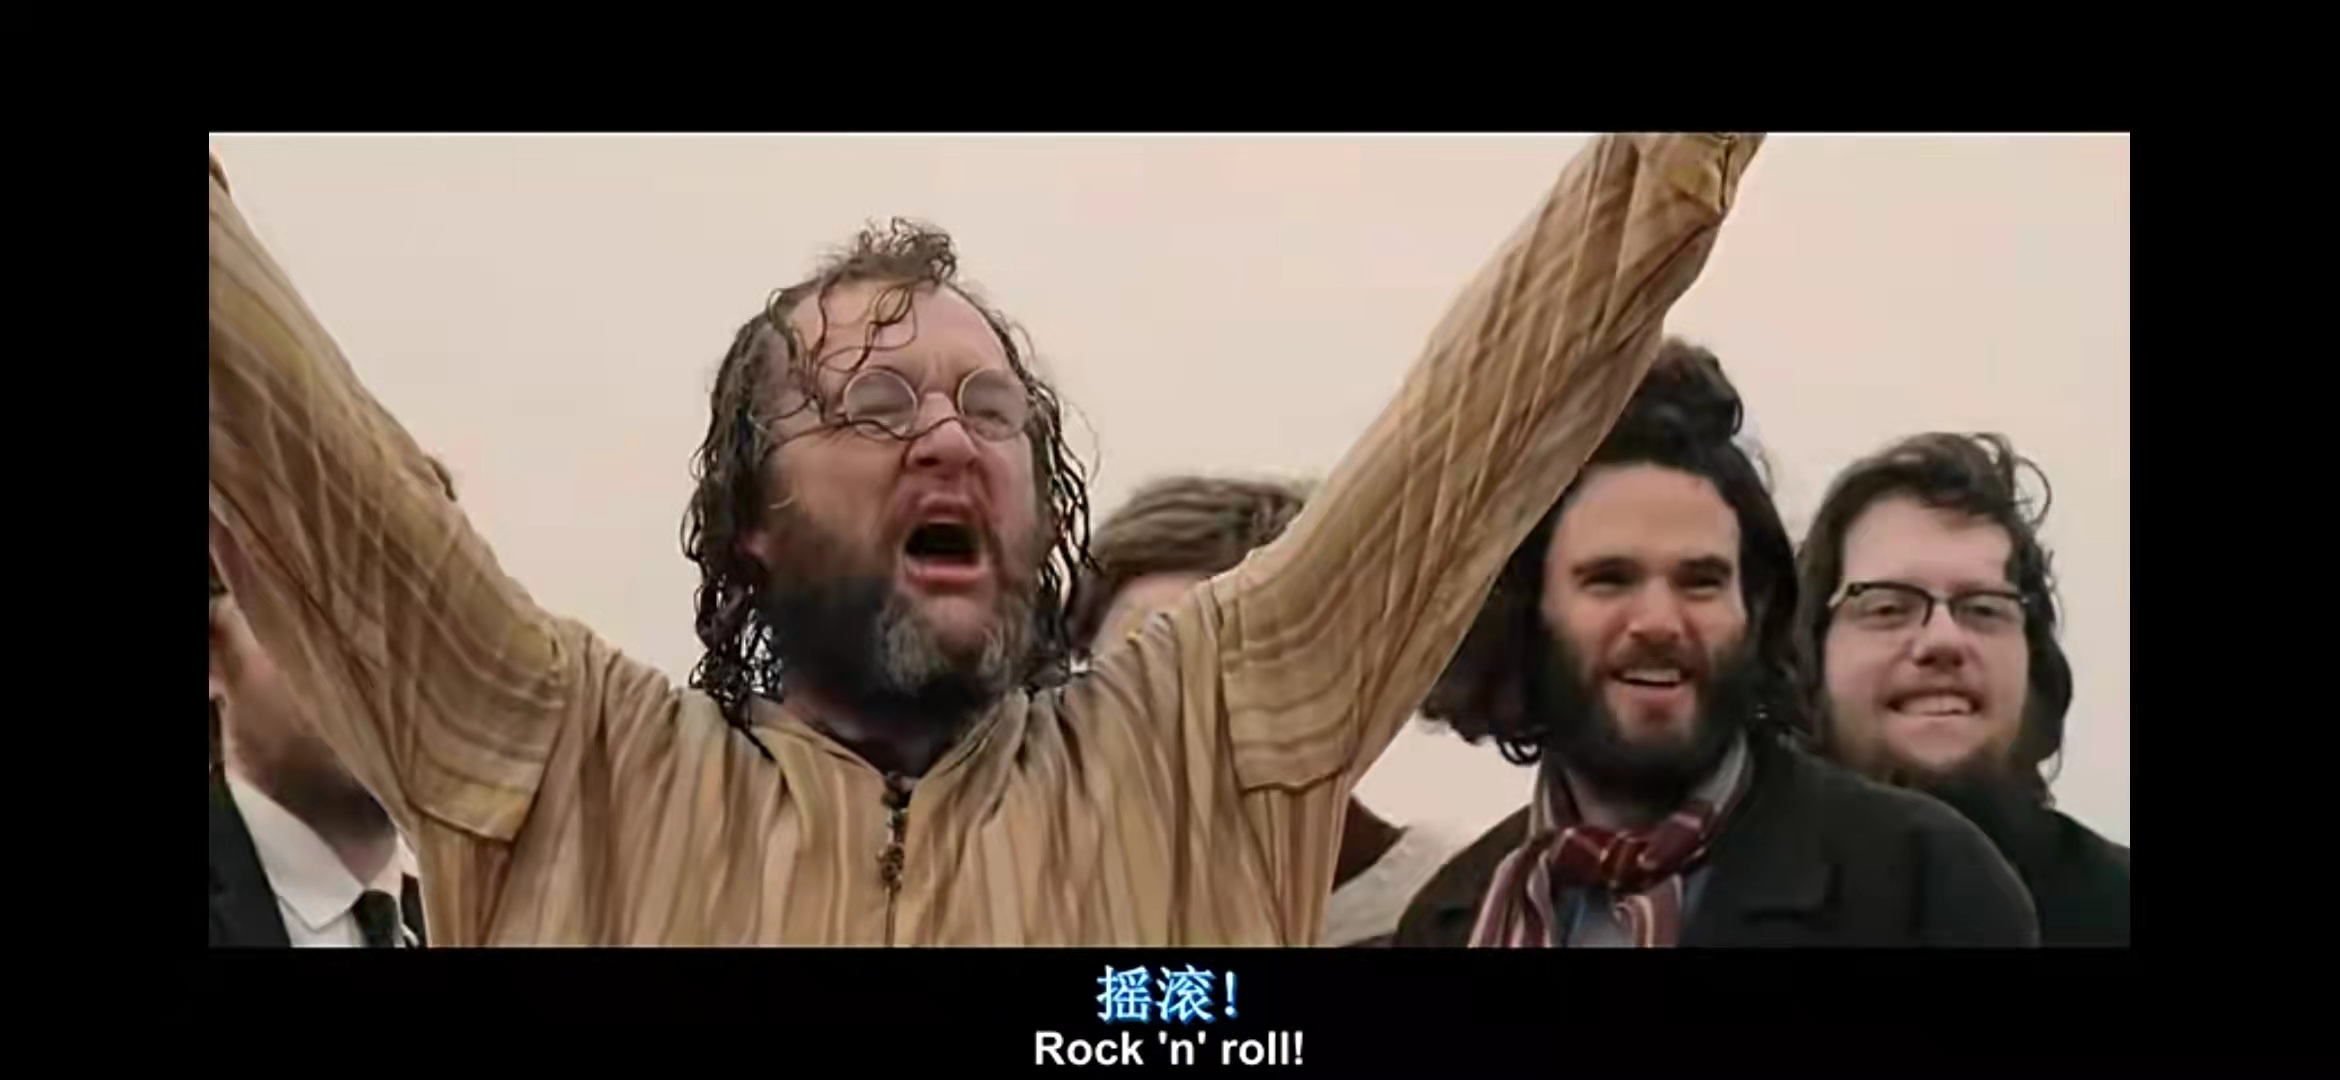
\includegraphics[scale=0.1]{fig/4}\label{3}
		}
		\quad
		\subfigure[磁化率与温度的关系图]{
			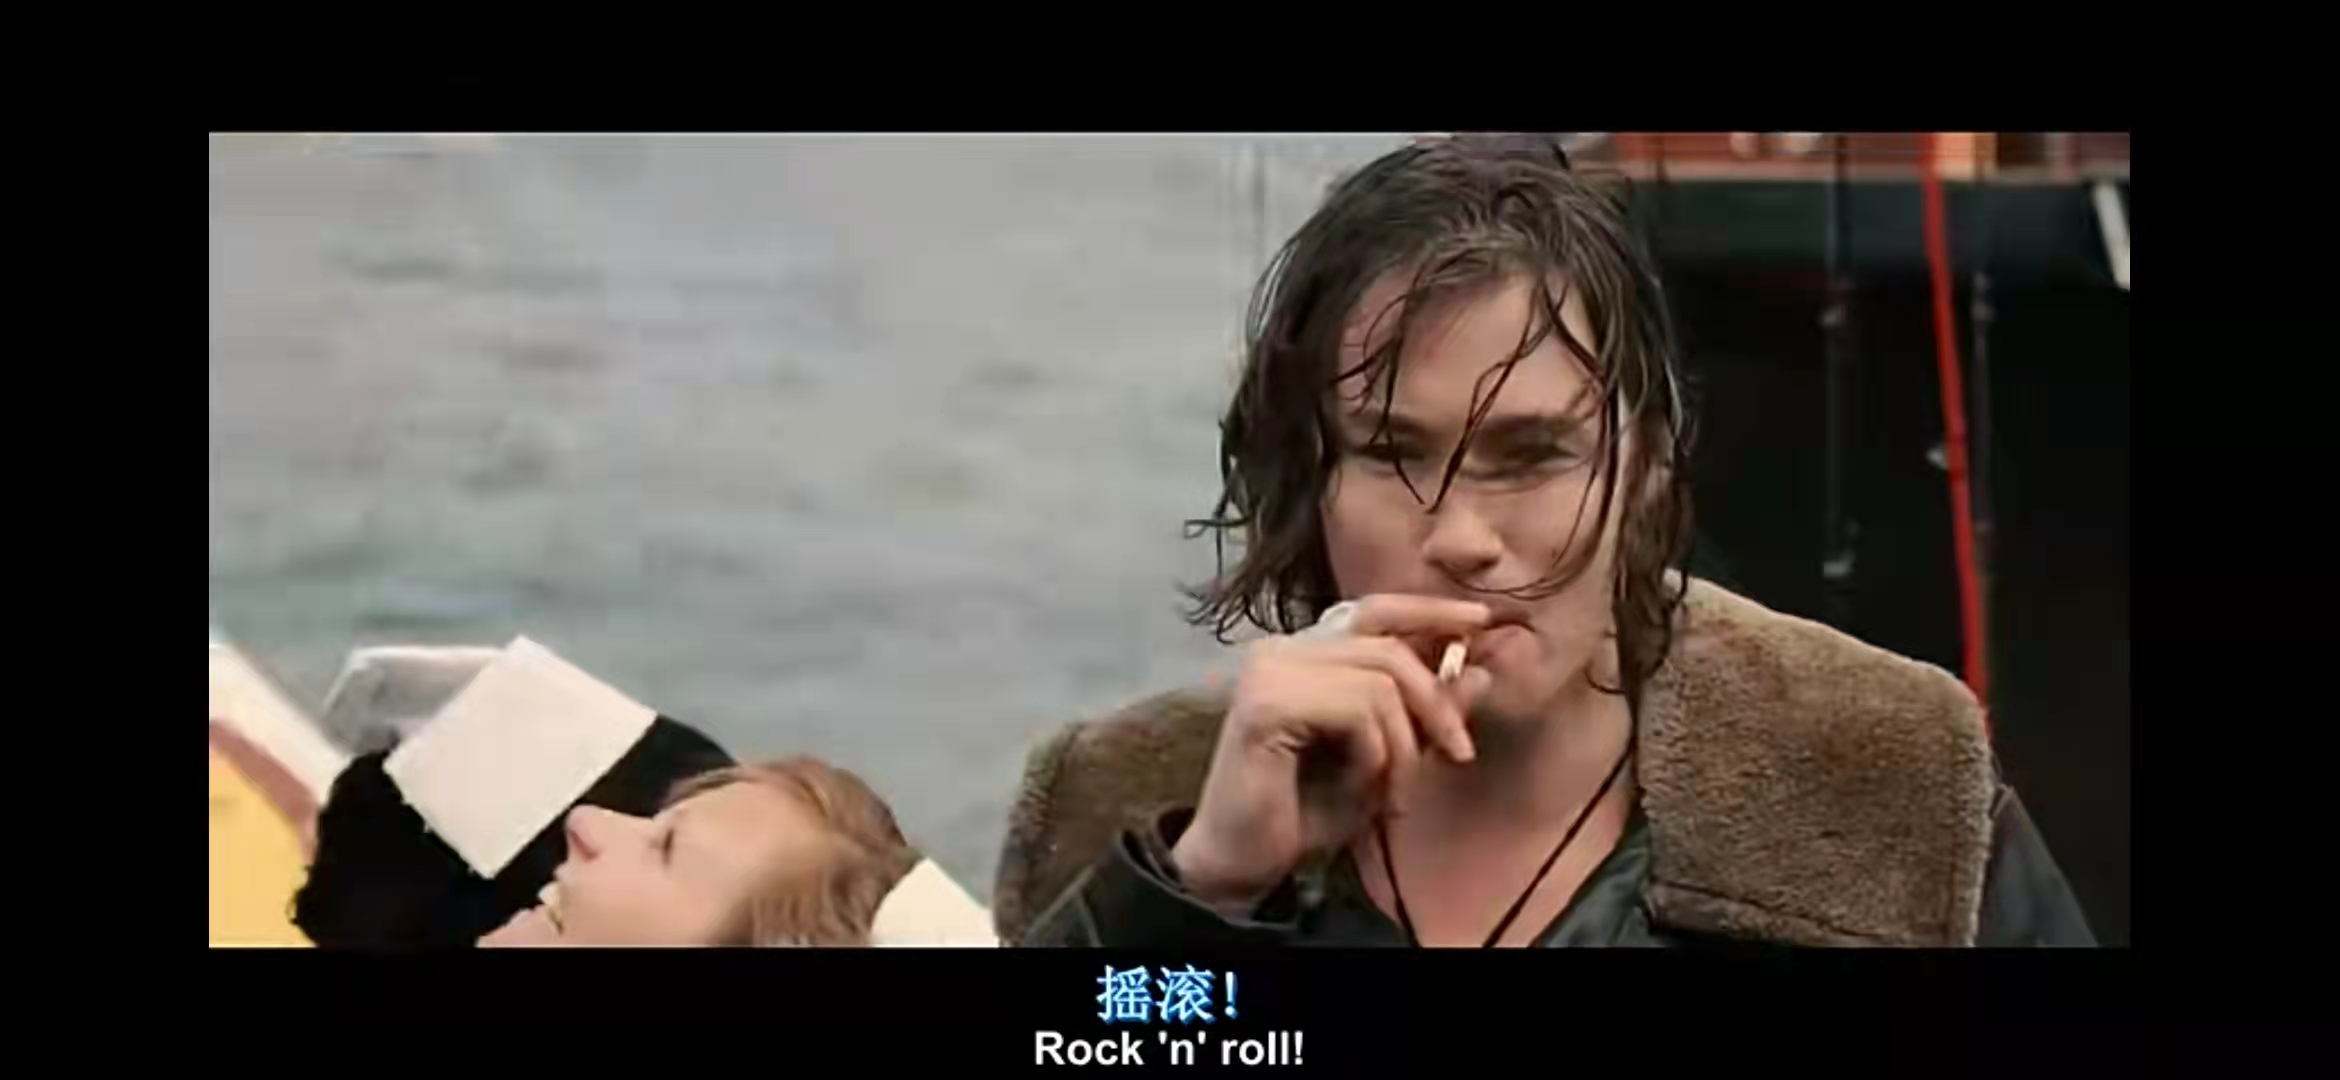
\includegraphics[scale=0.1]{fig/5}\label{4}
		}
		\caption{热力学量随时间变化曲线图} %四个子图组成的图片的批注
	\end{figure}

	\section{文献引用}
	我也不知道写啥随便写写。
	
	
	反对称交换作用,也称为Dzyaloshinskii-Moriya相互作用,是两个相邻磁自旋 ${  \mathbf {S} _{i}}{  \mathbf {S} _{i}}$和 ${  \mathbf {S} _{j}}{  \mathbf {S} _{j}}$对总的磁交换相互作用的贡献。它是由Igor Dzyaloshinskii首先基于朗道唯象理论的基础上提出的。而Toru Moriya将自旋 - 轨道耦合定义为反对称交换相互作用的微观机制。定量的分析,在这里哈密顿量可以写作${  H_{DM}=\mathbf {D} _{ij}\cdot (\mathbf {S} _{i}\times \mathbf {S} _{j})}{  H_{DM}=\mathbf {D} _{ij}\cdot (\mathbf {S} _{i}\times \mathbf {S} _{j})}$。在磁序系统中,这样倾向于自旋倾斜形成平行或反平行的排列磁矩,这也是在反铁磁体系出现的自旋倾斜弱铁磁性的原因。
	
	正如Moriya的最初的文献中所讨论的那样\cite{moriya1960anisotropic},${  \mathbf {D} _{ij}}{  \mathbf {D} _{ij}}$ 向量的方向由对称性所限制。 考虑到两个相邻离子之间的磁相互作用由超交换机制通过单个第三离子(配体)转移的情况, ${  \mathbf {D} _{ij}}{  \mathbf {D} _{ij}}$ 的取向由通过简单的关系 ${  \mathbf {D} _{ij}\propto \mathbf {r} _{i}\times \mathbf {r} _{j}=\mathbf {r} _{ij}\times \mathbf {x} }{  \mathbf {D} _{ij}\propto \mathbf {r} _{i}\times \mathbf {r} _{j}=\mathbf {r} _{ij}\times \mathbf {x} }$来决定。[3][4] 这意味着 ${  \mathbf {D} _{ij}}{  \mathbf {D} _{ij}}$ 取向垂直于由所涉及的三个离子跨越的三角形。 ${  \mathbf {D} _{ij}=0}{  \mathbf {D} _{ij}=0}$ 如果三级离子共线。
	
	反对称交换对于理解最近发现的多铁性类中的磁感应极化非常重要:这里,配位离子的小位移可以通过磁有序来诱导,因为系统倾向于消耗晶格能量来增强磁相互作用能量。这种机制被称为“逆Dzyaloshinskii-Moriya效应”。 在某些磁结构中,所有配体离子都向相同方向移动,导致极化。
	
\bibliographystyle{gbt7714-2005}
\bibliography{ref} 
\end{document}